\documentclass[10pt,a4paper]{article}
\usepackage[utf8]{inputenc} % para poder usar tildes en archivos UTF-8
\usepackage[spanish]{babel} % para que comandos como \today den el resultado en castellano
\usepackage{a4wide} % márgenes un poco más anchos que lo usual
\usepackage[conEntregas]{Sty/caratula}
\usepackage{Sty/mathtools}
\usepackage{Sty/float}
\usepackage[pdftex]{graphicx}
\usepackage{caption}
\usepackage{subcaption}
\usepackage[ruled,vlined,linesnumbered]{Sty/algorithm2e}
%Esto de abajo es para encabezado y pie de pagina
\usepackage{Sty/lastpage}
\usepackage{fancyhdr}
\usepackage{amsfonts}
\usepackage[noend]{algpseudocode}
\usepackage{enumerate} % AGREGO PARA PODER ENUMERAR LAS LINEAS DEL ALGORITMO
\usepackage{wrapfig}
\usepackage{amsmath}
\usepackage{verbatim}
\usepackage{listings}
\usepackage{color}
\usepackage{dsfont}


\definecolor{dkgreen}{rgb}{0,0.6,0}
\definecolor{gray}{rgb}{0.5,0.5,0.5}
\definecolor{mauve}{rgb}{0.58,0,0.82}

\lstset{frame=tb,
  language=Java,
  aboveskip=3mm,
  belowskip=3mm,
  showstringspaces=false,
  columns=flexible,
  basicstyle={\small\ttfamily},
  numbers=none,
  numberstyle=\tiny\color{gray},
  keywordstyle=\color{blue},
  commentstyle=\color{dkgreen},
  stringstyle=\color{mauve},
  breaklines=true,
  breakatwhitespace=true,
  tabsize=3
}

\pagestyle{fancy}


\cfoot{\thepage /\pageref{LastPage} }


\begin{document}

\fecha{\today}
\materia{Algoritmos y estructuras de datos III}
\titulo{Trabajo Práctico I}

\integrante{Cristian Gast\'on L\'opez}{515/08}{kakoseguro@hotmail.com}
\integrante{Fabio Seminara}{375/12}{faseminara@hotmail.com}
\integrante{Mat\'ias Millass\'on}{131/13}{matiasmillasson@gmail.com}
\integrante{Lautaro Leonel Alvarez}{268/14}{lautarolalvarez@gmail.com}

\maketitle
\newpage
\tableofcontents	

\newpage
\section{Problema 1: Cruzando El puente}
\subsection{Introducción}
El problema trata sobre un un grupo de arqueólogos y caníbales que quieren cruzar un puente pero se encuentran con el problema de que solo disponen de una sola linterna para cruzarlo. Solo pueden cruzar como mucho dos personas y no pueden dejar que los caníbales sean mayoría en ningún momento pues estos últimos se los comerían. \\

Para ejemplificarlo mejor vamos a mostrar una imagen representando una posible instancia del problema:


%\begin{figure}
%	\centering
%	\includegraphics[width=1.5cm]{images/canibalesYArqueologos.png}
%	\caption{Ejemplo de posible instancia.}
%\end{figure}

\begin {figure} [H]
\begin {center}
 \includegraphics[width=0.8\textwidth,natwidth=610,natheight=642]{images/canibalesYArqueologos.png}
 \caption{Ejemplo de posible instancia.}
\end {center}
 \end{figure}

Dada esta situacion inicial, vamos a intentar ejemplificar como es el mecanismo para resolver esta instancia y asi explicar de que se trata el problema.

Tenemos 6 personas, 2 caníbales y 3 arqueólogos. Cada uno de estos tiene una velocidad asociada y sabemos que las personas pueden pasar de grupos de a dos o de a uno, si los que pasan son dos entonces la velocidad de cruzado es igual a la velocidad del más lento de los dos, además también hay que tener en cuenta que la linterna es una sola y por lo tanto tiene que volver para poder seguir cruzando. Otra cosa a tener en cuenta es que en ninguno de los dos lados del puente puede haber mas caníbales que arqueologos (pués se los comerían), en el único caso que puede llegar a pasar esto es cuando hay solo caníbales y ningún arqueólogo ya que no tendrían a quién comerse.

Siguiendo con el ejemplo, en el paso 1 vamos a intentar llevar un grupo de dos, con la persona mas rápida para aprovechar su velocidad a la hora de volver con la linterna. El tema de elegir con quien ir en cada paso es fundamental, ya que si se elige por ejemplo dos caníbales, obligatoriamente vamos a tener que traer dos arqueólogos y volver con un caníbal, ya que de otra forma los caníbales serían mayoría del otro lado del puente.

Seguimos entonces por llevar un caníbal y un arqueólogo. Notar que en ningún momento se deja mas caníbales que arqueólogos. Eso es algo a tener en cuenta. Es por eso que es necesario saber bien a quién vamos a ir pasando y quién es el que va a volver con la linterna.
En los siguientes pasos se va dando prioridad a que vuelva el de mayor velocidad ya que (metiéndonos también un poco en la resolución) de esta forma, aprovechamos que vuelve solo y es la persona que menos tarda en cruzar el puente.

\subsection{Resoluci\'on}
Para la resolución vamos permutando las instancias pero con la restricción del enunciado, que es sólo poder mandar una o dos personas desde donde esta la linterna hacia el otro lado, pasando la linterna también.\\
La instancia inicial es: todas las personas de un mismo lado y la linterna a la izquierda. \\
Usamos la técnica de backtracking, la instancia inicial sería la raíz, y vamos bajando a medida que permutamos. El primer problema que se presenta es cómo no repetir permutaciones en una misma rama para no entrar en una rama infinita, para ésto cada padre va agregando a su hijo al conjunto de instancias, y le pasas este conjunto en la recursión al hijo. Cuando el hijo vuelve de la recursión el padre lo saca del conjunto (por si la permutación se repite pero en otra rama o sub-rama a partir del padre).

\subsubsection{Justificaci\'on de la soluci\'on}

\textbf{Identificación de cada instancia de manera única}: 
Cada instancia consiste de: una lista de persona en la izquierda, una lista de personas en la derecha y si la linterna esta en la izquierda o en la derecha.
Además podemos identificar cada instancia sólo mirando la lista izquierda y dónde está la linterna (no es necesario además mirar la lista derecha ya que dado un grupo de personas iniciales y dos listas izquierdas iguales, las listas de la derecha deben ser iguales). 
\newline
\newline
Para identificar cada instancia de una forma numérica usamos la escritura en binario. Inicialmente a cada persona le asignamos una \emph{ID} distinta, empezando en $0$ e incrementándola en uno por cada persona.
\\
Luego, armamos un arreglo de $n + 1$ elementos, siendo $n$ la cantidad inicial de personas. En este arreglo vamos a poner en la posición $i$ un $1$ o un $0$ si la persona con \emph{ID} $i$ está en la izquierda o si está en la derecha, respectivamente. En la posición $n$ hacemos lo mismo pero para la linterna.
De esta manera nos queda la representación en binario de un número al que vamos a usar para identificar a cada instancia.
   \newline
   \newline
   \textbf{Estructura del backtracking}:
   Para entrar a la raíz del árbol, y a los demás nodos nos metemos con esta función, que se llama una vez:
\begin{verbatim}
Recursión(Lista izq, Lista vacia, int tiempoOptimo, int tiempoActual, bool linternaIzq, Conjunto instancias, Arreglo instancia_actual)
\end{verbatim}   
Donde:
\begin{itemize}
\item izq: Es la lista de personas que están en la izquierda, en el caso inicial están todas las personas con sus números primos ya asignados
\item der: Van a estar todos los que están en la derecha, en el caso inical está vacía.
\item tiempoOptimo: En esta  variable nos vamos guardando el tiempo óptimo, al principio vale cero, y mientras valga 0 no habremos llegado a ninguna solución aún (Si al volver de toda la recursión sigue siendo cero, es porque no se puedo encontrar ninguna solución al problema inicial)
\item tiempoActual: Nos vamos guardando el tiempo que vamos sumando a medida que pasamos personas al otro lado, inicialmente es 0.  
\item instancias: es un conjunto tipo árbol que vamos manteniendo a medida que bajamos por la rama. Es decir, el padre inserta el ID del hijo al que va a saltar la recursión, y lo borra cuando el hijo vuelve, para así poder bajar por otra rama de instancias. \\ Es necesario que el padre borre al hijo del conjunto cuando éste vuelve, ya que al bajar por otra rama está bien que se repitan instancias de otras sub-ramas, porque sería una solución distinta. 
\item instancia\_actual: es el arreglo que nos sirve para identificar la instancia de la que venimos y así actualizarla para pasársela a la siguiente llamada.
\end{itemize}

\textbf{Cada vez que entramos a un nodo tenemos:}
\begin{lstlisting}
    IF (No hay personas del lado izquierda) 
        return minimo(tiempo optimo, tiempo actual); 
        
    ELSE IF(tiempo actual > tiempo optimo) return tiempo optimo;
\end{lstlisting}
\begin{itemize}
\item Chequeamos si en esta instancia no tenemos personas en la izquierda, es decir llegamos a una solución. En es caso afirmativo devolvemos el mínimo entre el tiempo óptimo (el tiempo que tardó la mejor solución que tenemos hasta ahora) y el tiempo actual (tiempo que nos tomó llegar hasta esta instancia).
\item Si el tiempo actual es mayor que el tiempo óptimo quiere decir que las soluciones que encontremos a partir de este nodo van a ser peores de lo que ya tenemos. Por lo tanto no vale la pena seguir bajando por el árbol. 
\end{itemize}

\textbf{Armar la instancia "hijo"}:

\textbf{Estrategia 1}:
\begin{itemize}
\item Linterna derecha: La instancia siguiente la armamos mandando de a uno hacia la izquierda, cuando ya recorrimos la lista derecha de esa forma, empezamos a mandar de a uno hacia la izquierda.
\item Linterna izquierda: Idem que lo anterior pero de de izquierda a derecha.  

\end{itemize}

      \textbf{Estrategia 2}:
\begin{itemize}
\item Linterna derecha: La instancia siguiente la armamos mandando de a uno hacia la izquierda, cuando ya recorrimos la lista derecha de esa forma, empezamos a mandar de a dos hacia la izquierda.
\item Linterna izquierda: En este caso comenzamos a mandar de a dos, y luego mandamos de a uno. Esto lo hacemos porque en todas las soluciones que intentamos a mano, en ninguna había que mandar de a dos personas de izquierda a derecha, por lo tanto nos pareció pertinenter mandar así para poder llegar a una primera solución de manera mas rápida. \\ Sin embargo puede ser que en algún problema haya que mandar de a uno de izquierda a derecha, entonces también tenemos que intentar buscar esa posible solución.  

\end{itemize}
      \textbf{Estrategia 3}:
\begin{itemize}
\item Esta estrategia es igual a la anterior, salvo que cuando mandamos de a una persona no recorremos toda la lista de lo que podemos mandar, si no que mandamos al caníbal mas rápido y luego al arqueólogo mas rápido. 
Sea una solución no óptima $S$ y una instancia de el algoritmo para llegar a $S$ en la que mandamos a una persona $P$. Asumiendo que $P$ es arqueólogo entonces mandando a otro arqueólogo $P'$ llegamos a otra solución $S'$. En particular elegimos a $P'$ como al arqueólogo mas rápido de los que están del lado de la linterna.
 
Como $tiempo(P')$ $\leq$ $tiempo(P)$ entonces al pasarlo al otro lado en $S'$ sumamos menos tiempo que al pasar $P$ en $S$. 
En alguna instancia posterior puede que $P'$ vuelva con otra persona $T$, pero como $P'$ es mas rápido que $P$, entonces el tiempo de pasar a estos dos es: $max(tiempo(P'),$ $tiempo(T))$ $\leq$ $max(tiempo(P),$ $tiempo(T))$.

Por lo tanto el costo de $S'$ es mejor o igual que el costo de $S$, y así nos armamos una solución mejor.
\end{itemize}
En cada caso actualizamos el arreglo que identifica a la instancia actual poniendo un $0$ o un $1$ en la posición de la $ID$ de la persona que mandamos a la derecha o a la izquierda. Además en la última posición actualizamos si la linterna se va a la derecha o a la izquierda.
\newpage
\textbf{Pasar al siguiente nodo}:
Una vez armada la instancia siguiente, calculamos el tiempo máximo de la ó las personas que mandamos, para sumárselo al tiempo actual.
\begin{lstlisting}
    tiempo actual += tiempo max(personas que pasan)

    ID Instancia = Numero(arreglo instancia_actual) 				

    IF( Izquierda es valida & Derecha es valida & !Pertenece(ID Instancia, instancias){	
			
          Agregar(ID Instancia, instancias)
				
          tiempo optimo = Recursion( Izquierda, Derecha, tiempo optimo, tiempo actual, !linterna actual, instancias, arreglo instancia_actual);
				
          Borrar(ID Instancia, instancias)
    }
    tiempo actual-= tiempo max(personas que pasan);	
\end{lstlisting}

\begin{itemize}
\item Al principio sumamos al tiempo actual el máximo de las dos o una personas que tenemos para mandar.
\item \begin{verbatim}
ID Instancia = Numero(arreglo instancia_actual) 				
\end{verbatim}
Nos guardamos en $instID$ el valor numérico de la instancia, calculando en base diez el numero en binario representado en el arreglo de instancia actual.
\item \begin{verbatim}
IF( Izquierda es valida & Derecha es valida & !Pertenece(ID Instancia, instancias){	
\end{verbatim}
Chequeamos si nos quedó una instancia válida, o sea mas arqueólogos que caníbales o sólo caníbales, en cada lado. Y también si la instancia que armamos ya la repetimos mas arriba en la rama, fijandonos si está en el conjunto de instancias. \\ Como explicamos antes, repetir instancias en una misma rama no tendría sentido para la solución óptima e incluso tendríamos una rama infinita. 
\item \begin{verbatim}
          Agregar(ID Instancia, instancias)
				
          tiempo optimo = Recursion( Izquierda, Derecha, tiempo optimo, tiempo actual, !linterna actual, instancias, arreglo instancia_actual);
				
          Borrar(ID Instancia, instancias)
				
\end{verbatim}
Cómo la instancia es válida y no está repetida en la rama, entonces la agregamos al conjunto de instancias por las que ya pasamos.\\
Luego nos metemos en la recursión con lo que tenemos y al volver sacamos la instancia del conjunto de instancias de la rama, esto es para que no influya en otras ramas distintas o sub-ramas de este nodo. 
\item Por último arreglamos el tiempo actual restándole el tiempo que habíamos sumado de las personas que mandamos, para que siempre quede el tiempo actual del nodo actual. 
\end{itemize}

\textbf{Nota:} Cuando volvemos a la primer recursión original, nos fijamos si el tiempo optimo es $0$, en ese caso no llegamos a ninguna solución y devolvemos $-1$, si no, devolvemos el tiempoOptimo.

\subsection{Cota de Complejidad}
Puede estimarse una cota superior acotando groseramente una rama, y así obteniendo la altura del árbol. \\
Ya que lo único que hacemos es ir permutando las instancias a medida que bajamos por una rama, mirando toda la rama puedo tener todas las permutaciones posibles de la lista inicial junto con la linterna. Esta cantidad es la suma de combinatorios de ir tomando de a dos elementos, de a tres, etc. Todo esto multiplicado por $2$ por la linterna.
Entonces, siendo A la altura del árbol y $n$ la cantidad de personas: 
\[A = 2 * \sum_{i=1}^{n}\binom  {n} {i}\ = 2 * (\sum_{i=0}^{n}\binom  {n} {i}\ -1) = 2 * ((\sum_{i=0}^{n}\binom  {n} {i} *1^{n-i} * 1^{i})\ - 1) = 2 * ((1 + 1)^n\ - 1) = 2 * (2^n - 1)
\]
\\
Para obtener la cantidad de hojas, falta calcular la cantidad de hijos que tiene un nodo. Como vamos mandando de a una persona, y luego de a dos, es claro que cada nodo tiene $\binom{n}{1}$ $+$ $\binom{n}{2}$ $=$ $n + (n*(n-1))/2$ $=$ $((n^2 + n)/2)$ hijos. \\
Por lo tanto la cantidad de hojas es: $((n^2 + n)/2)^{A}$
\\
\\
El costo en cada nodo es: 
\begin{itemize}
\item $\mathcal{O}(3n)$ por clonar dos listas y el arreglo de la instancia.
\item $\mathcal{O}(n + n + log(n))$ por fijarse si una instancia es válida, sacar la ID de la instancia y fijarse en el conjunto de instancias si no es repetida.
\item $\mathcal{O}(2log(n))$ por agregar y borrar sobre el conjunto de instancias recorridas. 
\item En total la suma de todos estos costos es $\mathcal{O}(n)$
\end{itemize}
\textbf{Cota total}:
Por lo tanto la complejidad total es $\mathcal{O}(((n^2 + n)/2)^A) *\mathcal{O}(n)$ $=$ $\mathcal{O}((n^2)^A*n)$ $=$ $\mathcal{O}(n^{2A+1})$ % Open at top left 
\subsection{Experimentación}

\par Para realizar pruebas sobre el algoritmo implementado, dividimos los casos de entrada en 3 tipos:
\begin{itemize}
	\item \textbf{Iguales:} Todas las velocidades de las personas son iguales. Para realizar las pruebas las seteamos todas en 10, pero este valor es anecdótico, ya que no influye realmente en el rendimiento del programa.
	\item \textbf{Pocas Diferencias:} Las velocidades de las personas varían en un rango acotado. Nos pareció interesando testear casos donde la diferencia de velocidades no sea grande. Para las pruebas seteamos valores entre 10 y 20.
	\item \textbf{Algunas Diferencias:} Las velocidades de las personas varían en un rango mucho mayor al caso anterior, pero sigue siendo un rango acotado. Este caso es interesante para verificar las podas agregadas al algoritmo y como utiliza estas diferencias de velocidades para descartar casos. Para realizar las pruebas tomamos los valores 10 y 500 y los repartimos entre las personas.
	%\item \textbf{Uno Muy Diferente:} La velocidad de uno difiere mucho con la del resto de las personas. Este caso también es interesando de ver para verificar que las podas realmente sirvan. Para realizar las pruebas le asignamos a una persona el valor 500 y al resto el valor 10.
\end{itemize}

\par Para cada uno de los casos mecionados vamos a correr todas las combinaciones de personas diez veces cada caso. Mediremos el tiempo de ejecución y tomaremos la mediana de estos valores para evitar outliers y otros inconvenientes. Luego observaremos y analizaremos los resultados.

\begin {figure} [H]
\begin {center}
 \includegraphics[width=1\textwidth,natwidth=610,natheight=642]{images/iguales.png}
 \caption{Caso donde todos tienen la misma velocidad.}
\end {center}
 \end{figure}
 \begin {figure} [H]
\begin {center}
 \includegraphics[width=1\textwidth,natwidth=610,natheight=642]{images/pocas_diferencias.png}
 \caption{Caso con velocidades que tienen poca diferencia entre ellas.}
\end {center}
 \end{figure}
 \begin {figure} [H]
\begin {center}
 \includegraphics[width=1\textwidth,natwidth=610,natheight=642]{images/algunas_diferencias.png}
 \caption{Caso donde una mitad es diferente a la otra mitad.}
\end {center}
 \end{figure}
 %\begin {figure} [H]
%\begin {center}
 %\includegraphics[width=1\textwidth,natwidth=610,natheight=642]{images/ej1_uno_muy_diferente.png}
 %\caption{Caso Uno Muy Diferente.}
%\end {center}
 %\end{figure}
 
%\begin{figure}
%	\centering
%	\includegraphics[width=1\textwidth]{images/ej1_iguales.png}
%	\caption{Caso Iguales}
%	\label{fig:ej1_iguales}
%\end{figure}
%\begin{figure}
%	\centering
%	\includegraphics[width=1\textwidth]{images/ej1_pocas_diferencias.png}
%	\caption{Caso Pocas Diferencias}
%	\label{fig:ej1_pocas_diferencias}
%\end{figure}
%\begin{figure}
%	\centering
%	\includegraphics[width=1\textwidth]{images/ej1_algunas_diferencias.png}
%	\caption{Caso Algunas Diferencias}
%	\label{fig:ej1_algunas_diferencias}
%\end{figure}
%\begin{figure}
%	\centering
%	\includegraphics[width=1\textwidth]{images/ej1_uno_muy_diferente.png}
%	\caption{Caso Uno Muy Diferente}
%	\label{fig:ej1_uno_muy_diferente}
%\end{figure}


\par En los primeros tres gráficos  están plasmados los tiempos de ejecución de las distintas combinaciones de personas posibles en cada uno de los 3 casos mencionados previamente. 

\par Algo que podemos notar en el gráfico es que los picos mas altos se dan en combinaciones de personas con un tipo de persona (canibal o arqueólogo) igual a cero ó en casos de muchas personas. El resto de los casos se mantienen en un número similar. Vamos a ver estos dos casos que nombramos:

\begin{itemize}
	\item Caso con un valor igual a cero: \\
	Para este caso hay que remitirse a la condición mas importante que se debe respetar: \textit{No puede haber en ningún momento más personas del tipo canibal que del tipo arqueólogo en un mismo lado del puente}. Esta condición es muy relevante para este caso, ya que al ser la cantidad de uno de los dos tipos de personas igual a cero (no hay caníbales o no hay arqueólogos) entonces esta condición siempre se cumple. Lo cual nos lleva a que no hay casos que se puedan evitar (podar), se deben tomar todas las variantes posibles. Esto hace que su tiempo de ejecución se amplie notablemente.
	Podemos ver en los gráficos, que en los valores \textit{0,1}, \textit{0,2} y \textit{0,3} van en aumento, mientras que los valores \textit{0,5} y en \textit{0,6} ya son notáblemente grandes.
Es en estos casos donde notamos que la cota de complejidad depende en gran parte de la cantidad de personas, ya que todas las instancias son válidas y una rama no se va a cortar porque los caníbales se hayan comido a los arqueólogos.

	\item Caso con cantidad de personas cercana a 6: \\
	Observando los resultados se nota que otro pico en los tiempos de ejecución se da en la combinación `3 arqueólogos y 3 caníbales'. Este caso es particular porque la resolución del problema requiere que en un momento vuelvan dos personas, en vez de una como pasa generalmente. 
Casos como el de '$k$ arqs y $1$ caníbal' son similares a '$k+1$ arqs y $0$ caníbales', ya que en todos los casos tenemos la misma cantidad total de personas y todas las instancias son válidas (un sólo caníbal no puede invalidar una instancia.

\item Estrategias: En los casos que requieren mas tiempo computacional se ve como la estrategia $1$ le gana a la $0$. En la mayoría de las soluciones viaja una sola persona desde la derecha hacia la izquierda, salvo en el caso de 3 y 3 en el que un momento vuelven dos. La estrategia $1$ siempre prueba primero las soluciones donde viaja una persona de derecha a izquierda. Mientras que la estrategia $0$ empieza mandando de a dos, consiguiendo así todas soluciones sub-óptimas al principio. Entonces era esperable que la estrategia $1$ le gana a la $0$.
\\
La estrategia $2$ manda en un orden similar que la $1$, es decir, siempre comienza mandando de a dos de izquierda a derecha, y volviendo de a uno de derecha a izquierda. Con la salvedad de que cada vez que le toca mandar una persona de un lado a otro, siempre elije la mas rápida (primero del tipo caníbal y luego del tipo arqueólogo). Como explicamos en una sección anterior, esta estrategia consigue soluciones mejores mas rapidamente. 
En el gráfico se aprecia claramente como en todos los casos la estrategia $2$ es igual o mejor que la $1$, que ya de por sí era mejor que la $0$.  En los casos donde la complejidad es mayor se ve como la estrategia $2$ es bastante mejor que la $0$.
\end{itemize}



\newpage
\section{Problema 2: Problemas en el camino}
\subsection{Introducción}
% Describir detalladamente el problema a resolver dando ejemplos del mismo y sus soluciónes.
\par El problema a resolver se trata de una balanza que se encuentra desequilibrada y debemos, por medio de diversas pesas con las que contamos, devolverle el equilibrio.
\par La balanza, en un principio, se encontraba en equilibro. Quitaron una llave (de la cual conocemos su peso) de en uno de los platillos y la balanza se desequilibró. Por suerte, contamos con una serie de pesas con la particularidad de que todos sus pesos son potencias de 3 y no hay repetidas. Por lo tanto queremos determinar qué pesas se deben colocar en cada platillo para reestablecer el equilibrio.
\par Siendo mas específicos,  a partir de una entrada P = `Peso de la llave quitada' de tipo entero debemos encontrar una combinación de potencias de 3 multiplicadas por +1 o -1 nos de como resultado P. Esto se resume en:

\begin{equation}
	\forall P \in \mathds{N},\ P = \sum_{i = 0}^{n} 3^{i} * a_i
\end{equation}
\begin{flushright}
	con $a_i \in \{-1, 0 , +1\}$, según el caso\\
	para algún $n \in \mathds{N}_0$
\end{flushright}

\subsection{Idea General de Resolución}

\par Continuando con la notación utilizada en la introducción, vamos a describir el algoritmo que utilizamos para resolver el problema.
\par El valor \textit{n} (exponente máximo de las potencias de 3) que utilizaremos es $\lceil log_{3}(P) \rceil$ (el por qué de la elección de este valor se explicará en el \textit{Lema 2 del Ej2} en la subsección \ref{ssub: lema_ej2_1}).
\par El algoritmo, en primer lugar, determina cuál es el valor de $a_{n} \in \{-1,0,+1\}$. Esto lo hace quedándose con el que cumpla $| P - a_{n} * 3^{n} | < \frac{3^{n}}{2}$ (para comprender el por qué de este valor ver el \textit{Lema 1 del Ej2} en la subsección \ref{ssub: lema_ej2_2}). Luego, reemplaza a $P$ por $P - a_{n} * 3^{n}$ y a $n$ por $n - 1$ y se llama recursivamente con los valores actualizados de $P$ y $n$. Así, va determinando los valores de cada $a_{i}$ (desde $i=n$ hasta $i=0$).

\subsubsection{Ejemplo ej2:}

\par Veamos un ejemplo del funcionamiento del algoritmo. Tomamos como entrada el número $P = 12$, tenemos $n = \lceil log_{3}(12) \rceil = 3$. El algoritmo compara entre los 3 casos posibles para $a_{k}$ y calcula la diferencia con P:

\begin{itemize}
	\item $a_{3} = -1 \rightarrow  12 - (-1) * 3^{3} =$ \textbf{39}.
	\item $a_{3} = 0 \rightarrow  12 - (0) * 3^{3} =$ \textbf{12}.
	\item $a_{3} = +1 \rightarrow  12 - (+1) * 3^{3} =$ \textbf{-15}.
\end{itemize}
\par Como $\frac{3^{3}}{2} = 14,5$, se determina que $a_{3} = 0$. Se actualiza $P = 12$ y $n = n - 1$ y se realizan nuevamente los mismos pasos. Se comparan los 3 casos:

\begin{itemize}
	\item $a_{2} = -1 \rightarrow  12 - (-1) * 3^{2} =$ \textbf{21}.
	\item $a_{2} = 0 \rightarrow  12 - (0) * 3^{2} =$ \textbf{12}.
	\item $a_{2} = +1 \rightarrow  12 - (+1) * 3^{2} =$ \textbf{4}.
\end{itemize}
\par Ahora tenemos que $\frac{3^{2}}{2} = 4,5$, entonces se determina que $a_{2} = +1$. Se actualiza $P = 12 - (+1) * 3^{2} = 4$ y $n = n - 1$ y se continúa. Se comparan los 3 casos:

\begin{itemize}
	\item $a_{1} = -1 \rightarrow  4 - (-1) * 3^{1} =$ \textbf{7}.
	\item $a_{1} = 0 \rightarrow  4 - (0) * 3^{1} =$ \textbf{4}.
	\item $a_{1} = +1 \rightarrow  4 - (+1) * 3^{1} =$ \textbf{1}
\end{itemize}
\par En este caso tenemos $\frac{3^{1}}{2} = 1,5$, por lo tanto se determina que $a_{1} = +1$. Actualizamos $P = 3 - (+1) * 3^{1} = 0$. Como $P=0$, terminamos de determinar todos los valores $a_{i}$ necesarios. Entonces nos queda que $12 = (+1) * 3^{2} + (+1) * 3^{1}$.

\subsection{Presentación del algoritmo y demostración de correctitud}

\par Antes que nada, vamos a enunciar dos lemas que nos servirán para entender y demostrar el correcto funcionamiento del algoritmo.

\subsubsection{Lema 1 del Ej2:}
\label{ssub: lema_ej2_1}

\par Queremos probar que dado un $P \in \mathds{N}$ y dado un $k \in \mathds{N}_0$, si $|P| \leq \frac{3^{k+1}}{2} \Longrightarrow \exists a_k \in \{-1,+1,0\}$ tal que $|P + a_i * 3^{k}| \leq \frac{3^{k}}{2}$.

\bigskip

\textbf{Demostración:}
\par Dado $P \in \mathds{N}$, $k \in \mathds{N}_0$ tal que $|P| \leq \frac{3^{k+1}}{2}$. Tenemos 3 posibilidades:
\begin{itemize}
	\item Si $|P| \leq \frac{3^{k}}{2} \Longrightarrow$ cumple con $a_{k}=0$.

	\item Si $P > \frac{3^{k}}{2}$: sabíamos que $P \leq \frac{3^{k+1}}{2}$, entonces tenemos que
	\begin{equation}
		\frac{3^{k}}{2} < P \leq \frac{3^{k+1}}{2}
	\end{equation}
	Sumando $-1 * 3^{k}$ tenemos
	\begin{equation}
		\frac{3^{k}}{2} -1 * 3^{k} < P -1 * 3^{k} \leq \frac{3^{k+1}}{2} -1 \cdot 3^{k}
	\end{equation}
	\begin{equation}
		\Longleftrightarrow -\frac{3^{k}}{2} < P -1 * 3^{k} \leq \frac{3^{k}}{2}
	\end{equation}
	Concluimos entonces que
	\begin{equation}
		| P - a_{k} * 3^k | \leq \frac{3^k}{2}
	\end{equation}
	\begin{flushright}
		con $a_{k} = -1$
	\end{flushright}

	\item Si $P < -\frac{3^{k}}{2}$: sabíamos que $P \geq -\frac{3^{k+1}}{2}$, entonces tenemos que
	\begin{equation}
		-\frac{3^{k+1}}{2} \leq P < -\frac{3^{k}}{2}
	\end{equation}
	\par Sumando $+1 * 3^{k}$ tenemos
	\begin{equation}
		-\frac{3^{k+1}}{2} +1 * 3^{k} \leq P < -\frac{3^{k}}{2} +1 * 3^{k}
	\end{equation}
	\begin{equation}
		\Longleftrightarrow -\frac{3^{k}}{2} \leq P < \frac{3^{k}}{2}
	\end{equation}
	\par Concluimos entonces que
	\begin{equation}
		| P - a_{k} * 3^k | \leq \frac{3^k}{2}
	\end{equation}
	\begin{flushright}
		con $a_{k} = +1$
	\end{flushright}
\end{itemize}
\par De esta manera pudimos ver que en las 3 posibilidades se cumple el lema planteado.

\subsubsection{Lema 2 Ej2}
\label{ssub: lema_ej2_2}

\par Queremos probar que $P \leq \frac{3^{n + 1}}{2}$ con $n = log_{3}(P)\ \forall P \in \mathds{N}_{0}$.

\medskip

\textbf{Demostración:}
\par Tenemos $P \in \mathds{N}_{0}$. Queremos ver que cumple:

\begin{equation}
	P \leq \frac{3^{log_{3}(P) + 1}}{2}
\end{equation}
\begin{equation}
	\Longrightarrow P \leq \frac{3^{log_{3}(P)} * 3}{2}
\end{equation}
\begin{equation}
	\Longrightarrow P \leq \frac{P * 3}{2}
\end{equation}
\begin{equation}
	\Longrightarrow 0 \leq \frac{1}{2} * P
\end{equation}
\par Como $P \in \mathds{N}_{0}$, sabemos que se cumple. Por lo tanto tenemos que $P \leq \frac{3^{n + 1}}{2} \forall P \in \mathds{N}_{0}$ con $n = log_{3}(P)$. Notar que como $log_3(p) \leq  \lceil log_3(p) \rceil \Longrightarrow p \leq \frac{3^{log_{3}(P) + 1}}{2} \leq \frac{3^{\lceil log_{3}(P) \rceil + 1}}{2}$


\bigskip

\par Luego de los dos lemas planteados, podremos demostrar la correctitud del algoritmo usado. Para esto, veamos el pseudocódigo del algoritmo:

\medskip

\SetAlgoLined
\SetKwProg{Fn}{Function}{:}{EndFunction}
\begin{algorithm}[H]
	\label{algo: pseudocodigo_ej2}
	\Fn{DameCombinacion(P: int, exponente: int, listaPositivos: lista(int), listaNegativos: lista(int))}{
		\BlankLine
		\If{$exponente < 0$}{
			return
		}
		\BlankLine
		$potenciaActual \gets potencia[exponente]$\\
		\BlankLine
		\uIf{$| P - (+1) * potenciaActual | < \frac{3^{exponente}}{2}$}{
			\BlankLine
			agregar $exponente$ al principio de $listaPositivos$\\
			$P = P - (+1) * potenciaActual$
			\BlankLine
		}
		\uElseIf{$| P - (-1) * potenciaActual | < \frac{3^{exponente}}{2}$}{
			\BlankLine
			agregar $exponente$ al principio de $listaNegativos$\\
			$P = P - (-1) * potenciaActual$
			\BlankLine
		}
		\BlankLine
		$DameCombinacion$($P$, $exponente - 1$, $listaPositivos$, $listaNegativos$)
		\BlankLine
	}
	\caption{Función encargada de calcular el valor asignado al exponente pasado como parámetro, según el número pasado por parámetro.}
\end{algorithm}

\medskip

\par Analicemos el algoritmo siguiendo el pseudocódigo. En la linea 5 se obtiene la potencia de un arreglo que tiene todas las potencias necesarias. Luego se comparan los casos de $a_k$ (lineas 6, 9) según el criterio del \textit{Lema 1 del Ej2} (subsección \ref{ssub: lema_ej2_1}). Si el valor elegido es $+1$, se agrega el exponente a la lista de exponentes positivos y se actualiza el número $P$. En cambio si el valor elegido es $-1$, se agrega el exponente a la lista de exponentes negativos y se actualiza el número $P$. Si no entró en ninguno de los casos anteriores se determina que el valor de $a_{k}$ es 0. Esto lo podemos asegurar porque el lema nos decía que sí o sí uno de los 3 valores cumple la implicación, como ninguno de los otros dos casos cumplía, sabemos que el 0 si cumple. Luego se llama recursivamente con los valores $P$, $listaPositivos$, $listaNegativos$ y $exponente$ decrementado en 1.
\par Si $P$ y $exponente$ cumplen las condiciones necesarias ($| P | \leq \frac{3^{exponente+1}}{2}$), sabemos que al final de la función se realiza una llamada recursiva a sí misma con valores $P$ y $exponente$ que cumple $| P | \leq \frac{3^{exponente+1}}{2}$ (teniendo en cuenta que $exponente$ se disminuyó en 1). Por lo tanto, al ingresar a la función en la llamada recursiva cumple las condiciones necesarias. Este ciclo se da hasta que $exponente$ es menor que 0 y cuando ocurre eso por el lema 2 $exponente = 0 \Longrightarrow P \leq \frac{3^0}{2} = 0,5 \Longrightarrow P = 0$ y por ende luego de la \'ultima llamada recursiva no quedan m\'as exponentes por calcular. En este caso (en la linea 3) se termina la función.
\par Cabe destacar además, que para cada exponente la función solo se llama una vez. Esto nos asegura que los exponentes no se repitan y solo haya un $a_{k}$ asignado a un exponente.

\medskip

\par Volviendo un poco al problema planteado en la introducción, veamos como se utiliza la función planteada para resolverlo. Vamos a llamar a la función con los valores: $P$ = el peso de la llave; $exponente$ = $log_{3}(P)$; $listaPositivos$ y $listaNegativos$ dos listas vacías. Luego de que la función termine su ejecución (y sus respectivas llamadas recursivas), en las listas $listaNegativos$ y $listaPositivos$ estarán los valores de los exponentes necesarios para equilibrar la balanza.


\subsection{Cota de Complejidad}
%3. Deducir una cota de complejidad temporal del algoritmo propuesto (en funci´on de los par´ametros
%que se consideren correctos) y justificar por qu´e el algoritmo desarrollado para la resoluci´on del
%problema cumple la cota dada. Utilizar el modelo uniforme salvo que se explicite lo contrario.

\par Vamos a dar una cota de complejidad del algoritmo y analizaremos el por qué de ese valor. Para esto observaremos el pseudocódigo del Algoritmo \ref{algo: pseudocodigo_ej2}.
\par Veamos la función \textit{DameCombinacion}. En las linea 2-4 hay una comparación y la salida de la función de costo O(1). Luego, en la linea 5 hay una asignación de una exponencial que tiene costo O(1) dado que se accede a una posici\'on de un arreglo. Las guardas de las lineas 6 y 9 tienen costo O(1). En las lineas 7 y 10 se agregan dos enteros al inicio de dos listas. La implementación utilizada para esas listas nos asegura que esa acción tiene costo O(1). Luego en las lineas 8 y 11 se realizan dos asignaciones con costo O(1). Luego en la linea 12 se ejecuta la llamada recursiva. Por lo tanto, para una ejecución de la función (sin contar la llamada recursiva) se obtiene un costo de O(1).
\par Recordemos que la función es llamada con exponente $log_{3}(P)$, y este exponente se disminuye de a 1 antes de hacer una llamada recursiva. Entonces obtenemos una complejidad O($log_{3}(P)$) * O(DameCombinacion) = 0($log_{3}(P)$) * O(1) = 0($log_{3}(P)$).
\par Luego, para imprimir los resultados en el formato pedido, se recorren las listas $listaNegativos$ y $listaPositivos$. Esto nos lleva O(longitud($listaNegativos$) + longitud($listaPositivos$)). Pero sabemos que a lo sumo se recorren $log_{3}(P)$ exponentes y ninguno se repite, por lo que sabemos entonces que $longitud(listaNegativos) + longitud(listaPositivos) \leq log_{3}(P)$. Por lo tanto imprimir los resultados tiene costo O(log(P)).

\medskip

\par En conclusión, la cota de complejidad del algoritmo utilizado para resolver el ejercicio 2 es \textbf{O(log(P))}.

\medskip

\par Para este problema debíamos cumplir una cota de complejidad O($\sqrt{P}$). Dado que nuestra cota de complejidad es O(log(P))
queremos ver que $O(log(P)) \subset O(\sqrt(P))$.\\

Pasemos $P$ a variable real. veamos la relaci\'on de orden entre las respectivas derivadas \\
\begin{equation}
    (log_3(P))' = \frac{1}{P \cdot ln(3)}
\end{equation}
\begin{equation}
    (\sqrt(P))' = \frac{1}{sqrt(P)}\\
\end{equation}
Veamos que la ecuaci\'on 15 es mayor que la ecuaci\'on 14:
\begin{equation}
        \frac{1}{P \cdot ln(3)} \leq \frac{1}{sqrt(x)}\\
\end{equation}
\begin{equation}
        \Longrightarrow P \cdot ln(3) \geq sqrt(P)\\
\end{equation}

\begin{equation}
        \Longrightarrow \sqrt(P) \cdot ln(3) \geq 1\\
\end{equation}
Es f\'acil ver que la ecuaci\'on 18 se cumple $\forall P > 0$.
Como la derivada de $\sqrt(P)$ es mayor que la de $log_3(P)$ entonces 
\begin{equation}
        lim_{n \to \infty}\frac{log_3(P)}{\sqrt(P)} = 0
\end{equation}
Entonces $O(log(P)) \subset O(\sqrt(P))$ $\square$ \\
Por la demostraci\'on de arriba se cumpli\'o con la cota pedida.

\subsection{Experimentaci\'on}
Como se puede ver en la figura nuestra hipotesis de que la complejidad de nuestro algoritmo es $O(log(P))$ se verifica.

\begin{figure}
	\centering
	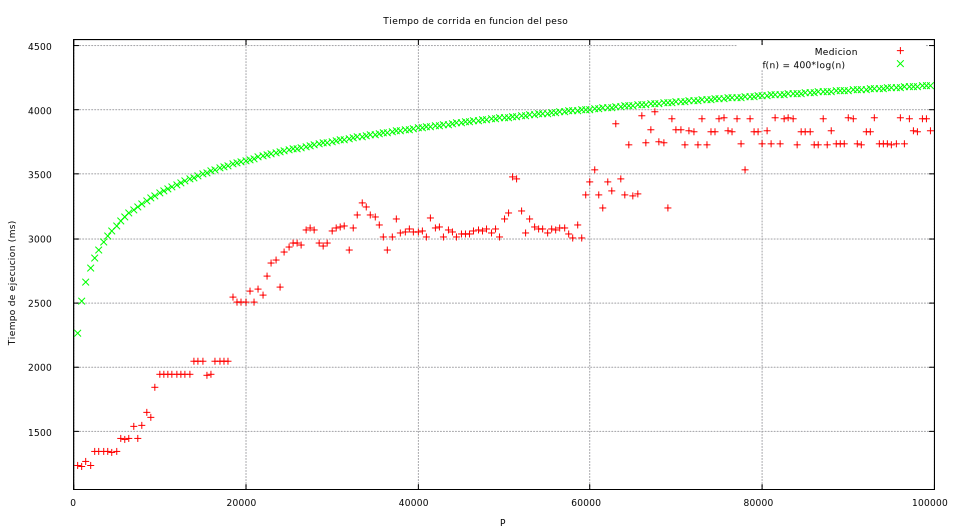
\includegraphics[width=1\textwidth]{images/graficoposta.png}
	\caption{Gr\'afico del tiempo de ejecuci\'on con respecto a $log(p)$}
	\label{}
\end{figure}



\newpage
\section{Problema 3: Guardando el tesoro}
\subsection{Introducci\'on}
% Describir detalladamente el problema a resolver dando ejemplos del mismo y sus soluciónes.
En este problema unos arque\'ologos quieren llevarse algunos tesoros, para esto tienen algunas mochilas (a lo sumo tres).
Los tesoros tienen un peso y un valor, y el objetivo es organizar los tesoros de tal manera que el valor total de los tesoros llevados sea el m\'aximo posible.
La dificultad radica en que la capacidad de las mochilas es limitada (podr\'ian tener distinta capacidad cada una).
Formalmente, dada una lista de tesoros representados como una tupla $(peso, valor)$ y m enteros $K_i$ representando la capacidad m\'axima de las mochilas (0 $<$ m $\leq$ 3),
se piden $m$ listas de tesoros tales que la sumatoria de los pesos de la $i$-\'esima lista sea menor o igual a $K_i$
y que la sumatoria de los valores de todos los tesoros de las $m$ listas sea el m\'aximo posible.

\subsection{Resoluci\'on}
%2. Explicar de forma clara, sencilla, estructurada y concisa, las ideas desarrolladas para la resoluci´on
%del problema. Para esto se pide utilizar pseudoc´odigo y lenguaje coloquial combinando adecua
%damente ambas herramientas (¡sin usar c´odigo fuente!). Se debe tambi´en justificar por qu´e el
%procedimiento desarrollado resuelve efectivamente el problema.
Este problema claramente es muy similar al \emph{knapsack problem}, pero con la variante de que hay varias mochilas para rellenar. \\
La t\'ecnica algor\'itmica utilizada es programaci\'on din\'amica. Podemos utilizar dicha t\'ecnica algor\'itmica porque se cumple el principio de optimalidad, dado que si tomo una secuencia $s$ de las decisiones que tom\'e sobre una subsecuencia de objeto cualesquiera (la decisi\'on trata sobre si lo puse en alguna mochila o no y en tal caso en cual coloqu\'e ese tesoro) tal que sea \'optima para nuestro problema. Entonces si a $s$ le quito la decisi\'on para el \'ultimo objeto esta subsecuencia de $s$ es \'optima para el problema con la capacidad de la mochila (correspondiente seg\'un mi decisi\'on) reducida en el peso del \'ultimo objeto. Notar que si esto no fuera as\'i, es decir que existiera una mejor soluci\'on para el problema con los objetos de la subsecuencia, entonces tambi\'en lo ser\'ia para todos los objetos ($s$). Como no asum\'i nada sobre $s$ esto se cumple cuando $s$ es la lista de tesoros.\\
La funci\'on recursiva que devuelve el valor m\'aximo posible, nosotros la
definimos as\'i: \\

\begin{equation*}
     max\_profit(i,m1,m2,m3) = \left\{
	       \begin{array}{ll}
		 0      & \mathrm{si\ } i < 0 \\
		 max( \\
		 peso(i) \leq m1 * (valor(i)+max\_profit(i-1,m1-peso(i),m2,m3)), \\
         peso(i) \leq m2 * (valor(i)+max\_profit(i-1,m1,m2-peso(i),m3)), \\
         peso(i) \leq m3 * 
         (valor(i)+max\_profit(i-1,m1,m2,m3-peso(i))), \\
         max\_profit(i-1,m1,m2,m3)\\
         ) & \mathrm{si no\ }  \\
	       \end{array}
	     \right.
\end{equation*}

Vamos a explicar esta funci\'on, el primer par\'ametro es el \'indice de la lista de tesoros y
los demas son los respectivas capacidades disponibles en cada mochila. Sabemos que formalmente la funci\'on deber\'ia tener como par\'ametro la lista
tesoros pero para simplificar hicimos ese abuso de notaci\'on. Tambi\'en se pide que el lector asuma definidas las funciones \"peso\"
y \"valor\" que devuelven respectivamente el peso y el valor del tesoro $i$-\'esimo de la lista.
Esta funci\'on en el caso base se fija si puede colocar el tesoro en alguna mochila y en ese caso devuelve el valor, si no lo puede colocar
devuelve 0. En el caso recursivo la funci\'on se fija el m\'aximo de cuatro casos. \'Estos son: coloco el objeto en la mochila 1, lo coloco en la 2, lo coloco en la 3 o no lo coloco en ninguna.
Notar que $f$ tambi\'en sirve en los casos en los que hay 1 o dos mochilas, sencillamente se ponen la capacidades en 0. \\
Como este algoritmo es de programaci\'on din\'amica adem\'as de definir la funci\'on recursiva tengo que decidir como voy a implementar la parte de la memoizaci\'on.
Los resultados parciales me los voy a guardar en una \"matriz\" que va a tener una dimensi\'on con los \'indices de cada tesoro y una dimensi\'on por cada mochila con las capacidades parciales posibles, es decir desde cero hasta la capacidad m\'axima de cada mochila.
En cada posici\'on de esta matriz voy a guardarme el beneficio m\'aximo con esas capacidades y la lista de tesoros desde cero hasta $i$ como as\'i tambi\'en desde que posici\'on de la matriz llegu\'e a ese m\'aximo.
Es decir, con cual de los 4 casos del max de max\_ profit obtuve dicho m\'aximo.
Nuestro algoritmo toma la entrada y hace una lista de tesoros. Luego calcula los beneficios parciales y el beneficio total (ver pseudoc\'odigo). Y para imprimir los tesoros colocados en cada mochila sencillamente nos situamos en el extremo de la matriz que tiene el \'ultimo objeto y las capacidades m\'aximas de las mochilas
dado que en esa casilla est\'a beneficio acumulado. Luego con los campos hijoWeight voy \"saltando\" a otras posiciones de la matriz hasta terminar de recorrer todos los objetos.


\subsubsection{Pseudoc\'odigo}
Antes del pseudoc\'odigo es oportuno aclarar que cada casillero de la matriz es una tupla de:\\
beneficio: int, \\
mochila: int, \\
visitado: bool, \\
hijoWeight1: int, \\
hijoWeight2: int, \\
hijoWeight3 : int \\

El campo mochila indica en que mochila puse el tesoro de esa posicion, los campos hijoWeight dan las \"coordenadas\" de la matriz desde donde calcule ese m\'aximo. Estos campos van a ser cruciales para imprimir la salida con el formato pedido.\\
Decidimos realizar dos implementaciones, una \emph{top down} o recursivo y la otra \emph{bottom up} o iterativa.

\subsubsection{Top down}
\medskip

\SetAlgoLined
\SetKwProg{Fn}{Function}{:}{EndFunction}
\begin{algorithm}[H]
	\label{algo: pseudocodigo_ej3}
	\Fn{knasack(matriz: Casilla[][][][], tesoros: lista(int,int), i: int, weight1: int, weight2: int, weight3: int)}{
		\BlankLine
		\If{$i < 0$}{
			return 0
		}
		\BlankLine
    \If{visite matriz[i][wieght1][weight2][weight3]}{
      return matriz[i][wieght1][weight2][weight3].beneficio
    }
    \Else{
      beneficios[4]\\
      \If{tesoros[i] entra en la mochila 1}{
        $beneficios[0] = valor(i) + knapsack(matriz, tesoros, i-1, weight1-peso(i), weight2, weight3)$
      }
      \If{tesoros[i] entra en la mochila 2}{
        $beneficios[1] = valor(i) + knapsack(matriz, tesoros, i-1, weight1, weight2-peso(i), weight3)$
      }
      \If{tesoros[i] entra en la mochila 3}{
        $beneficios[2] = valor(i) + knapsack(matriz, tesoros, i-1, weight1, weight2, weight3-peso(i))$
      }
      $beneficios[3] = knapsack(matriz, tesoros, i-1, weight1, weight2, weight3)$

      $indMax \gets indiceDelMaximo(beneficios)$

      actualizar la posicion matriz[i][weight1][weight2][weight3] segun indMax

      return matriz[i][wieght1][weight2][weight3].beneficio
    }
		\BlankLine
	}
	\caption{Función encargada de devolver el beneficio maximo y de poner valores en la matriz para luego imprimir los tesoros correspondientes a cada mochila}
\end{algorithm}

\medskip

Es f\'acil ver que knapsack computa la funci\'on max\_profit.
En esta implementaci\'on no necesariamente se calculan todas las posiciones de la matriz sino a\'olamente las que son necesarias.

\subsubsection{Bottom up}

\medskip

\SetAlgoLined
\SetKwProg{Fn}{Function}{:}{EndFunction}
\begin{algorithm}[H]
	\label{algo: pseudocodigo_ej3}
	\Fn{knasack(matriz: Casilla[][][][], tesoros: lista(int,int), weight1: int, weight2: int, weight3: int)}{
		\BlankLine
	  \For {cada tesoro}{
	    \For{j desde 0 hasta weight1 inclusive}{
	        \For{k desde 0 hasta weight2 inclusive}{
	            \For{k desde 0 hasta weight3 inclusive}{
	               actual $\gets$ tesoro[i] \\
	               beneficios[4]\\
	               \If{actual entra en la mochila 1}{
                   $beneficios[0] = actual.valor+ matriz[i-1][weight1-actual.peso][weight2][weight3]$
                   }
                   \If{actual entra en la mochila 2}{
                   $beneficios[1] = actual.valor + matriz[i-1][weight1][weight2-actual.peso][weight3])$
                   }
                   \If{actual entra en la mochila 3}{
                    $beneficios[2] = actual.valor + matriz[i-1][weight1][weight2][weight3-actual.peso]$
                   }
                    $beneficios[3] = matriz[i-1][weight1][weight2][weight3])$
                    $indMax \gets indiceDelMaximo(beneficios)$

                    actualizar la posicion actual de matriz segun indMax
                }
            }
	    }
	}
	

    return matriz[longitud(tesoros)][pesos[0]][pesos[1]][pesos[3]].beneficio
	\BlankLine
	}
	
	\caption{Función encargada de devolver el beneficio m\'aximo y de poner valores en la matriz para luego imprimir los tesoros correspondientes a cada mochila}
\end{algorithm}

\medskip

En esta versi\'on de la soluci''on se puede ver que el cuerpo del ciclo \emph{for} central (es decir, desde la l\'inea 6 hasta la 18) que son muy similares a las de la implementaci\'on top down. En dichas l\'ineas se encuentra la parte de decisi\'on de que es lo conveniente para lograr el beneficio m\'aximo porque computa la funci\'on $max\_profit$. La \'unica diferencia radica en que se llenan todas las posiciones de la matriz en orden.


\subsection{Cota de Complejidad}
%3. Deducir una cota de complejidad temporal del algoritmo propuesto (en funci´on de los par´ametros
%que se consideren correctos) y justificar por qu´e el algoritmo desarrollado para la resoluci´on del
%problema cumple la cota dada. Utilizar el modelo uniforme salvo que se explicite lo contrario.

\begin{itemize}
    \item Bottom up: Primero veamos el cuerpo del ciclo \'ultimo ciclo for. Se crea un arreglo de longitud 4 ($O(1)$), luego se hace una asignaci\'on y cuatro condicionales cuyas guardas se evaluan en $O(1)$ (s\'olo se realizan comparaciones entre enteros) y los cuerpos de cada condicional cuestan $O(1)$ tambi\'en porque lo \'unico que se hace es acceder a una posici\'on de la matriz, una suma y una asignaci\'on. Por ende el costo del cuerpo es $O(1)$. Luego el ciclo de la l\'inea 5 iteran $O(weight3)$ veces, el de la l\'inea 4 $O(weight2)$ y los otros dos $O(weight1)$ y $O(C)$ ($C$ es la cantidad de tesoros) respectivamente. Es importante recordarle al lector que si la cantidad de mochilas no es 3, los pesos m\'aximos de las mochilas que no existen valen $0$, por lo tanto en ese caso esos ciclos costar\'ian $O(1)$. Por \'ultimo el ciclo que dice en que mochila se colocaron los tesoros es $O(C)$. Dado que todos estos ciclos est\'an anidados la complejidad resultante es $O($ $\Sigma  K_{i}^{m}*C)$, con $K_i$ el peso m\'aximo que soporta la mochila i-\'esima, $m$ la cantidad de mochilas y $C$ la cantidad de objetos. 
    
    \item Top down:
    La complejidad de este algoritmo es $O($($\Sigma$ $K_{i})^m*C)$ donde $K_i$ es la capacidad de cada mochila, $m$ es la cantidad de mochilas y $C$ es la cantidad total de tesoros. Notar que cuando hay menos de tres mochilas los arreglos \"interiores\" tienen longitud 1, por ende no empeoran la complejidad.\\
    Nuestra justificaci\'on se basa en que necesitamos inicializar nuestro objeto Casilla de la matriz antes de llamar a la funci\'on knapsack. Eso tiene un costo de $O($($\Sigma$ $K_{i})^m*C)$. \\
    Luego cuando se llama a la funci\'on knapsack tambi\'en es $O($($\Sigma$ $K_{i})^m*C)$, dado que todos los llamados recursivos se guardan en la matriz. Entonces en el peor caso knapsack llena la matriz.
    Por \'ultimo el ciclo que dice en que mochila se colocaron los tesoros es $O(C)$. En las l\'ineas 2-22 se realizan varias asignaciones, accesos a posiciones de la matriz, comparaciones de enteros. Todas estas operaciones cuestan $O(1)$.
    
\end{itemize}



\subsection{Experimentación}

\par Vamos a realizar diversos experimentos sobre las implementaciones de los dos algoritmos mencionados previamente (Top down y Bottom up) con el fin de comparar sus rendimientos y poder sacar conclusiones sobre ellos.

\par Algunos experimentos miden tiempos y comparan estos resultados con la cota de complejidad antes planteada. Por esto, vamos a definir algunos parámetros que nos van a servir para entendernos mejor:

\begin{itemize}
	\item \textit{$N$}: Cantidad de tipos de tesoros.
	\item \textit{$M$}: Cantidad de mochilas.
	\item \textit{$K_i$}: Capacidad de la mochila $i$.
	\item \textit{$C_i$}: Cantidad de tesoros del tipo $i$.
	\item \textit{$\sum_{i = 1}^{N} C_i$}: Cantidad total de tesoros. A partir de ahora nos referiremos a esta sumatoria como \textit{C}.
	\item \textit{$\sum_{i = 1}^{M} K_i$}: Capacidad total de todas las mochilas. A partir de ahora nos referiremos a esta sumatoria como \textit{K}.
\end{itemize}

\par La cota de complejidad planteada es O($(\sum_{i = 1}^{M} K_i)^{M} \cdot (\sum_{i = 1}^{N} C_i)$), que con la notación tomada nos queda O($K^{M} \cdot C$).

\subsubsection{Experimento 1: $\#$ Tesoros y Capacidad total de mochilas en aumento}

\par En el primer experimento, fijaremos la cantidad de mochilas (\textit{M}) y variaremos la cantidad total de tesoros (\textit{C}) y la capacidad total de mochilas (\textit{K}) para ver cómo se comportan y si cumplen la cota de complejidad antes mencionada.

\par Tomaremos M=1. Por lo tanto, la cota de complejidad nos queda O($K_1 \cdot C$). Vamos a ir aumentando los valores de $K_1$ y $C$ y tomaremos el tiempo que le toma al programa encontrar la solución y finalizar. Tanto la cantidad de tipos de tesoros, como los pesos y los valores de cada tipo de tesoro serán tomados al aleatoriamente en un rango entre 1 y $K_1$ (para que siempre pueda entrar en la mochila). Aumentaremos el valor $K_1$ mas rápidamente que $C$, para que al menos varios tesoros puedan entrar en la mochila (sabiendo que su peso está acotado por la capacidad de esta mochila).

\par Esperamos que, para ambas implementaciones, los tiempos se mantengan en un orden lineal con respecto a $K_i \cdot C$. Creemos que la implementación \textit{Bottom up} debe mantenerse con tiempos mayores con respecto a la implementación \textit{Top down}, ya que la primera va a calcular todas las casillas de la matriz, mientras que la segunda solo va a completar las necesarias.

\begin{figure}[H]
	\centering
	\includegraphics[width=0.9\textwidth]{Problema3/img/exp1_tiempos_general.png}
	\caption{Resultados del experimento 1.}
	\label{fig: exp1_tiempos_general}
\end{figure}

\par En la figura \ref{fig: exp1_tiempos_general} podemos ver los resultados del experimento. Sobre el eje x ubicamos el valor $K_1 \cdot C$ para poder observar si el gráfico de los tiempos obtenidos es de orden lineal. Notamos que en ambas implementaciones el orden efectivamente es lineal, aunque multiplicado por una constante muy baja. Podemos decir que las diferencias esperadas entre las implementaciones se cumplieron: \textit{Bottom up} se mantuvo siempre por encima de \textit{Top down}.

\subsubsection{Experimento 2: Tesoros con peso 1}

\par Para este experimento, vamos a partir del experimento 1 y le haremos ciertos cambios. Mantendremos fija la cantidad de mochilas (M = 1) y variaremos la cantidad de tesoros y la capacidad de la mochila. El cambio mas importante es que tomaremos siempre peso=1, para todos los tesoros. También tomaremos siempre $K_1 = C$.

\par Lo que queremos ver al tomar esta caracterización de la entrada, es un peor caso de la implementación \textit{Top down}. Esto se lo adjudicamos a que debe recorrer un porcentaje de la matriz mayor al del resto de los casos, ya que la cantidad de capacidades a las que puede llegar (como combinación de poner o no los objetos anteriores) es mayor. Veamos un ejemplo: nos ubicamos en la casilla M[i,j], donde \textit{i=número de tesoro} y \textit{j=capacidad disponible en la mochila}. Podemos agregar el tesoro a la mochila o no agregarlo. Como el tesoro tiene peso=1, debemos pasar a las casillas M[i+1,j] y a la M[i+1,j-1]. Podemos ver que no se saltean filas, porque los pesos son siempre 1. De esta forma se recorre un mayor porcentaje de casilleros. Si entramos en detalle se recorrerán exáctamente $\sum_{i=1}^{K_1}i = \frac{K_i \cdot (K_1 + 1)}{2}$ casilleros (no creemos que venga al caso la demostración, simplemente es un dato informativo).

\begin{figure}[H]
	\centering
	\includegraphics[width=0.9\textwidth]{Problema3/img/exp2_tiempos_peor.png}
	\caption{Resultados del experimento 2.}
	\label{fig: exp2_tiempos_peor}
\end{figure}

\par En la figura \ref{fig: exp2_tiempos_peor} podemos ver los resultados del experimento 2. Podemos ver que los tiempos de la implementación \textit{Top down} se mantienen por debajo de \textit{Bottom up}, a pesar de que creimos que este era un peor caso, y que podía influir en el rendimiento. Igualmente, los resultados se corresponden con lo esperado, ya que \textit{Bottom up} siempre recorre y calcula toda la matriz, mientras que habíamos mencionado que \textit{Top down} (en este caso) recorre $\frac{K_i \cdot (K_1 + 1)}{2}$ casilleros.

\par Antes de comparar los distintos casos para cada implementación veamos el siguiente experimento.

\subsubsection{Experimento 3: Tesoros muy pesados}

\par En el experimento 2 fijamos el peso en 1, haciendo que el algoritmo \textit{Top down} recorra gran parte de la matriz. En este experimento vamos a hacer lo contrario, fijaremos los pesos en un valor alto para que no pueda entrar en la mochila y se recorra muy poca parte de la matriz. Esto se lo adjudicamos al hecho de que al no poder colocar ningún tesoro en la mochila solo recorre una fila de la matriz. Veamos un ejemplo: nos ubicamos en la casilla M[i,j], donde \textit{i=número de tesoro} y \textit{j=capacidad disponible en la mochila}. No podemos agregar el tesoro a la mochila (por su peso), entonces solo podemos movernos a la casilla M[i+1,j]. De esta manera solo se recorre una fila: $C$ casillas.

\par Tomaremos una mochila (M=1), fijaremos el peso de cada tesoro en $K_i$+1 y veremos qué pasa con el rendimiento al ir aumentando $C$ y $K_1$.

\begin{figure}[H]
	\centering
	\includegraphics[width=0.9\textwidth]{Problema3/img/exp3_tiempos_mejor.png}
	\caption{Resultados del experimento 3.}
	\label{fig: exp3_tiempos_mejor}
\end{figure}

\par En la figura \ref{fig: exp3_tiempos_mejor} podemos ver los resultados del experimento. Notamos que los tiempos de la implementación \textit{Top down} son menores a los de los experimentos previos, pero no notamos una gran diferencia. Además, un dato interesante es que los tiempos de la implementación \textit{Bottom up} también disminuyeron. No sabemos concrétamente a qué se debe esto. Creemos que es porque al no entrar en algunas condiciones (por el excesivo peso de los tesoros) se evita algunas asignaciones y llamadas a funciones. Al tomarse tamaños de matriz tan grandes, tal vez este factor afecte levemente el rendimiento y esto sea lo que vemos reflejado en los resultados de los experimentos.

\par Ahora si, con estos últimos experimentos podemos comparar los resultados agrupándolos por implementación.

\begin{figure}[H]
	\centering
	\includegraphics[width=0.9\textwidth]{Problema3/img/comparacion_td.png}
	\caption{Experimentos 2 y 3 - Top Down.}
	\label{fig: comparacion_td}
\end{figure}

\begin{figure}[H]
	\centering
	\includegraphics[width=0.9\textwidth]{Problema3/img/comparacion_bu.png}
	\caption{Experimentos 2 y 3 - Bottom Up.}
	\label{fig: comparacion_bu}
\end{figure}

\par En la figura \ref{fig: comparacion_td} podemos ver las diferencias entre el experimento 2 (nuestro peor caso) y el experimento 3 (nuestro mejor caso) en la implementación \textit{Top down}. Para el caso de la implementación \textit{Bottom up} se puede observar la figura \ref{fig: comparacion_bu}. Como mencionamos anteriormente, no creemos que esos casos sean mejores ni peores. Si creemos que hay factores que influyen levemente y se ven reflejados en el gráfico.

\subsubsection{Experimento 4: Medición de memoria}

\par Quedo claro que la implementación \textit{Top down} es mejor en cuanto a tiempos de ejecución que \textit{Bottom up}. Pero sabemos que la implementación \textit{Top down} se basa en una función que se llama recursivamente muchas veces hasta lograr calcular la solución al problema y creemos que esto puede impactar diréctamente sobre la memoria utilizada al momento de ejecutarse. Por lo tanto, en este experimento vamos a comparar la memoria utilizada por ambas implementaciones.

\par Vamos a enfocarnos en el peor caso de \textit{Top down} (experimento 2). La única diferencia será que no mediremos el tiempo de ejecución, sino la memoria utilizada. Para medir esta memoria utilizaremos funciones de java (\textit{Runtime}) que nos dan la memoria utilizada por el programa antes de ser administrada por el garbage collector.

\par Esperamos que en este caso, la mejor performance la tenga la implementación \textit{Bottom up}, ya que \textit{Top down} realiza muchas llamadas recursivas y acumulará muchos datos en el heap.

\begin{figure}[H]
	\centering
	\includegraphics[width=0.9\textwidth]{Problema3/img/exp4_memoria.png}
	\caption{Resultados del experimento 4.}
	\label{fig: exp4_memoria}
\end{figure}

\par En la figura \ref{fig: exp4_memoria} podemos ver los resultados del experimento. Notamos que, a partir de un valor entre los 50000 y 100000, la implementación \textit{Top down} consume mas memoria que \textit{Bottom up}. Igualmente, esperábamos una diferencia mayor. No creemos que esta diferencia sea tan importante como para contrarestar los buenos resultados obtenidos en cuanto a tiempos de ejecución.

\smallskip

\par Luego de experimentar con las implementaciones, debemos decir que \textit{Top down} obtuvo una diferencia favorable en cuanto a tiempos y no se sobrepasó mucho en cuanto a memoria utilizada. Si debemos quedarnos con una implementación creemos que esta sería la elegida.

\newpage
\section{Modificaciones}
\par En general, reevimos todo el informe y las implementaciones y modificamos las partes en las cuales recibimos correcciones y las partes que consideramos que debían mejorarse.

\par A continuación vamos a enunciar algunos cambios y correcciones del TP1 que creemos que son relevantes y es importante nombrarlas.

\subsection{Ejercicio 1: Cruzando el puente}

\begin{itemize}
	\item Se hicieron modificaciones generales en el informe. Se corrigieron errores mencionados en la corrección y se trató de ampliar las explicaciones detallando mejor los conceptos y ejemplificando de mejor manera.
	\item Se mejoró la explicación de los algoritmos, así como su pseudocódigo.
	\item Se implementaron podas se explicaron y se experimentó teniendo en cuenta estas estrategias.
\end{itemize}

\subsection{Ejercicio 2: Problemas en el camino}

\begin{itemize}
	\item Se corrigieron detalles de implementación.
	\item Se agregó la sección de experimentación, que era un faltante del TP1.
\end{itemize}

\subsection{Ejercicio 3: Guardando el tesoro}

\begin{itemize}
	\item Se mejoraron las explicaciones del informe.
	\item Se implementaron dos algoritmos, uno top down y otro bottom up. Esto por una corrección surgida en el coloquio del TP1.
	\item Se explicaron ambos algoritmos y se dieron las cotas de complejidad.
	\item Se experimentó comparando estas implementaciones y con distintos casos de entrada.
\end{itemize}

\newpage
\section{Anexo}
\subsection{C\'odigo Cruzando el puente}
	\begin{lstlisting}
package soluciones;

import java.util.LinkedList;
import java.util.Scanner;
import java.util.TreeSet;

import utils.Persona;

public class Ejercicio1{


	public static void main(String[] args){
		
		long time_start, time_end;
		time_start = System.currentTimeMillis();
		
		Ejercicio1 e = new Ejercicio1();
        
        
		Scanner capt = new Scanner(System.in);
        int estrategia = capt.nextInt();
        int N_arqs = capt.nextInt();
        int M_canis = capt.nextInt();
        capt.nextLine();
        LinkedList<Persona> inicial = new LinkedList<Persona>();
       
        
        while(N_arqs > 0){
        	Persona p = new Persona("A", capt.nextInt());
        	inicial.add(p);
        	N_arqs--;
        }

        capt.nextLine();
        while(M_canis > 0){
        	Persona p = new Persona("C", capt.nextInt());
        	inicial.add(p);
        	M_canis--;
        }
        capt.close();

        //int estrategia= 2;
        //System.out.println(e.Resolver(inicial,estrategia));
        int asd = e.Resolver(inicial,estrategia);
        //System.out.println("termine");
		time_end = System.currentTimeMillis();
		System.out.println(time_end - time_start);
	}
	
	@SuppressWarnings("unchecked")
	private int Resolver(LinkedList<Persona> iniciales, int tipo_estrategia){
		int tiempoMax = -1;/*Pensar una cota maxima para los iniciales*/

		int k = 0;
		for(Persona p : iniciales){	//Seteo las ids con numeros primos.
			p.setID(k);
			k++;					
		}
		
		Integer[] arr_instancia = new Integer[iniciales.size() + 1]; //Arreglo que indentifica la instancia actual personas mas linterna
		for(int i = 0; i < arr_instancia.length; i++){
			arr_instancia[i] = 1; //Estan todos en la izquierda, inclusive la linterna.
		}
		boolean linternaIzq = true;	//Solo por motivos declarativos
		LinkedList<Persona> vacia = new LinkedList<Persona>();
		LinkedList<Persona> izq = (LinkedList<Persona>) iniciales.clone();	//Clono para no arruinar la lista original.
		
		TreeSet<Integer> instancias = new TreeSet<Integer>();
		instancias.add(sacarID(arr_instancia));			//Agrego a la raiz como instancia.
		
		int res = -1;

		
		if(tipo_estrategia == 0) res = auxResolver0(izq, vacia, tiempoMax, 0, linternaIzq, instancias, arr_instancia);
		else if(tipo_estrategia == 1) res = auxResolver1(izq, vacia, tiempoMax, 0, linternaIzq, instancias, arr_instancia);
		else if(tipo_estrategia == 2) res = auxResolver2(izq, vacia, tiempoMax, 0, linternaIzq, instancias, arr_instancia);
		
		return res;
	}

@SuppressWarnings("unchecked")
private int auxResolver0(LinkedList<Persona> izq, LinkedList<Persona> der, int tiempoOptimo, int tiempoActual, boolean linternaIzq, TreeSet<Integer> instancias, Integer[] instancia_actual){
		
		/*CON LA ESTRATEGIA 0 SIEMPRE EMPIEZO MANDANDO UNO DE LOS DOS LADOS, Y LUEGO DOS*/
		
		if(izq.size() == 0) return minimo(tiempoOptimo, tiempoActual);	//Si la lista izquierda vino vacia es porque llegue a una solucion

		else if(maximo(tiempoOptimo, tiempoActual) == tiempoActual) return tiempoOptimo;	//Si tiempoActual es mas grande que el optimo no sigo
		
		
		
		boolean mandarUno = true; //Mando uno sii estoy en la derecha o en la izquierda pero con un solo tipo.
		boolean termine = false;

		int i = 0;
		int j = 1;
		Persona persona1;
		Persona persona2;

		int tMAX;
		do{
			
			Integer[] aux_instanciaActual = instancia_actual.clone();					
			
			
			LinkedList<Persona> auxIzq = (LinkedList<Persona>) izq.clone();
			LinkedList<Persona> auxDer = (LinkedList<Persona>) der.clone();

			if(linternaIzq){	//Si linterna esta en izquierda saco uno de la izquierda
				aux_instanciaActual[aux_instanciaActual.length-1] = 0;
				
				persona1 = izq.get(i);

				auxIzq.remove(i);
				aux_instanciaActual[persona1.dameID()] = 0;
				
				
				auxDer.add(persona1);
			}
			else { 	//Idem con derecha
				aux_instanciaActual[aux_instanciaActual.length-1] = 1;

				persona1 = der.get(i);

				auxDer.remove(i);
				aux_instanciaActual[persona1.dameID()] = 1;
				
				auxIzq.add(persona1);
			}

			tMAX = persona1.dameTiempo();

			if(mandarUno){	//Si tenia que mandar uno actualizo el indice y mas;
				i++;
				if(i == izq.size() && linternaIzq){
					mandarUno = false;
					i = 0;
					if(izq.size()==1) termine = true;
				}
				else if (i == der.size() && !linternaIzq){
					mandarUno = false;
					i = 0;
					if(der.size()==1) termine = true;
				}

			}

			else{		//Si tenia que mandar 2 tengo que sacar otro de donde este la linterna y actualizar los indices.
				if(linternaIzq) {
					persona2 = izq.get(j);
					auxIzq.remove(j-1);
					aux_instanciaActual[persona2.dameID()] = 0;

					
					auxDer.add(persona2);
					
				}
				else {
					persona2 = der.get(j);
					auxDer.remove(j-1);
					aux_instanciaActual[persona2.dameID()] = 1;
					
					auxIzq.add(persona2);
				}
				j++;

				if((linternaIzq && j == izq.size()) || (!linternaIzq && j == der.size())){	//Si j llego al final tengo que avanzar el i y seguir mandando.
					i++;
					j = i+1;
				}

				if(i==izq.size()-1 && linternaIzq){	//Si i llego al final es porque termine de mandar 2
					termine = true;

				}
				else if(i==der.size()-1 && !linternaIzq){
					termine = true;
				}

				tMAX = persona2.dameTiempo() > tMAX ? persona2.dameTiempo() : tMAX;

			}

			tiempoActual+= tMAX; //Sumo lo que cuesta este viaje.
			
			
			Integer instID = sacarID(aux_instanciaActual);			//calculo el ID de la nueva instancia				
			if(valido(auxIzq) && valido(auxDer) && !instancias.contains(instID)){	//Si la instancia nuva no es valida, o ya la repeti en esta rama, no sigo bajando.
			
				instancias.add(instID);	//Agrego la instancia "hijo" al conjunto 
				
				tiempoOptimo = auxResolver0( auxIzq, auxDer, tiempoOptimo, tiempoActual, !linternaIzq, instancias, aux_instanciaActual);
				
				instancias.remove(instID);	//Saco la instancia "hijo" anterior porque voy a bajar por otra rama.
			}
			tiempoActual-=tMAX;	//Arreglo el tiempoActual;

		}while(!termine);
		
		return tiempoOptimo;

	}


	@SuppressWarnings("unchecked")
	private int auxResolver1(LinkedList<Persona> izq, LinkedList<Persona> der, int tiempoOptimo, int tiempoActual, boolean linternaIzq, TreeSet<Integer> instancias, Integer[] instancia_actual){
		
		/*Con la ESTRATEGIA 1 siempre que estoy a la izquierda empiezo mandando de a dos y siempre que estoy a la derecha empiezo mandando de a uno*/
		
		if(izq.size() == 0) return minimo(tiempoOptimo, tiempoActual);	//Si la lista izquierda vino vacia es porque llegue a una solucion 

		else if(maximo(tiempoOptimo, tiempoActual) == tiempoActual) return tiempoOptimo;	//Si tiempoActual es mas grande que el optimo no sigo
		
		
		
		boolean mandarUno = !linternaIzq || (linternaIzq && izq.size() == 1); //Mando uno sii estoy en la derecha o en la izquierda pero con un solo tipo.
		boolean termine = false;

		int i = 0;
		int j = 1;
		Persona persona1;
		Persona persona2;

		int tMAX;
		do{
			
			Integer[] aux_instanciaActual = instancia_actual.clone();					
			
			
			LinkedList<Persona> auxIzq = (LinkedList<Persona>) izq.clone();
			LinkedList<Persona> auxDer = (LinkedList<Persona>) der.clone();

			if(linternaIzq){	//Si linterna esta en izquierda saco uno de la izquierda
				aux_instanciaActual[aux_instanciaActual.length-1] = 0;
				
				persona1 = izq.get(i);

				auxIzq.remove(i);
				aux_instanciaActual[persona1.dameID()] = 0;
				
				
				auxDer.add(persona1);
			}
			else { 	//Idem con derecha
				aux_instanciaActual[aux_instanciaActual.length-1] = 1;

				persona1 = der.get(i);

				auxDer.remove(i);
				aux_instanciaActual[persona1.dameID()] = 1;
				
				auxIzq.add(persona1);
			}

			tMAX = persona1.dameTiempo();

			if(mandarUno){	//Si tenia que mandar uno actualizo el indice y mas;
				i++;
				if(i == izq.size() && linternaIzq){
					termine = true;
				}
				else if (i == der.size() && !linternaIzq){
					mandarUno = false;
					i = 0;
					if(der.size()==1) termine = true;
				}

			}

			else{		//Si tenia que mandar 2 tengo que sacar otro de donde este la linterna y actualizar los indices.
				if(linternaIzq) {
					persona2 = izq.get(j);
					auxIzq.remove(j-1);
					aux_instanciaActual[persona2.dameID()] = 0;

					
					auxDer.add(persona2);
					
				}
				else {
					persona2 = der.get(j);
					auxDer.remove(j-1);
					aux_instanciaActual[persona2.dameID()] = 1;
					
					auxIzq.add(persona2);
				}
				j++;

				if((linternaIzq && j == izq.size()) || (!linternaIzq && j == der.size())){	//Si j llego al final tengo que avanzar el i y seguir mandando.
					i++;
					j = i+1;
				}

				if(i==izq.size()-1 && linternaIzq){	//Si i llego al final es porque termine de mandar 2
					mandarUno = true;
					i=0;
				}
				else if(i==der.size()-1 && !linternaIzq){
					termine = true;
				}

				tMAX = persona2.dameTiempo() > tMAX ? persona2.dameTiempo() : tMAX;

			}

			tiempoActual+= tMAX; //Sumo lo que cuesta este viaje.
			
			
			Integer instID = sacarID(aux_instanciaActual);			//calculo el ID de la nueva instancia				
			if(valido(auxIzq) && valido(auxDer) && !instancias.contains(instID)){	//Si la instancia nuva no es valida, o ya la repeti en esta rama, no sigo bajando.
			
				instancias.add(instID);	//Agrego la instancia "hijo" al conjunto 
				
				tiempoOptimo = auxResolver1( auxIzq, auxDer, tiempoOptimo, tiempoActual, !linternaIzq, instancias, aux_instanciaActual);
				
				instancias.remove(instID);	//Saco la instancia "hijo" anterior porque voy a bajar por otra rama.
			}
			tiempoActual-=tMAX;	//Arreglo el tiempoActual;

		}while(!termine);
		
		return tiempoOptimo;

	}

	
	@SuppressWarnings("unchecked")
	private int auxResolver2(LinkedList<Persona> izq, LinkedList<Persona> der, int tiempoOptimo, int tiempoActual, boolean linternaIzq, TreeSet<Integer> instancias, Integer[] instancia_actual){
		
		/* ESTRATEGIA 2 ES IGUAL A LA 1, SALVO QUE CUANDO MANDO UNA PERSONA, MANDO AL MINIMO */
		if(izq.size() == 0) return minimo(tiempoOptimo, tiempoActual);	//Si la lista izquierda vino vacia es porque llegue a una solucion 

		else if(maximo(tiempoOptimo, tiempoActual) == tiempoActual) return tiempoOptimo;	//Si tiempoActual es mas grande que el optimo no sigo
		
		
		
		boolean mandarUno = !linternaIzq || (linternaIzq && izq.size() == 1); //Mando uno sii estoy en la derecha o en la izquierda pero con un solo tipo.
		boolean termine = false;

		int tipo_mas_rapido = 0;
		int i = 0;
		int j = 1;
		Persona persona1;
		Persona persona2;

		int tMAX;
		do{
			
			Integer[] aux_instanciaActual = instancia_actual.clone();					
			
			
			LinkedList<Persona> auxIzq = (LinkedList<Persona>) izq.clone();
			LinkedList<Persona> auxDer = (LinkedList<Persona>) der.clone();

			if(linternaIzq){	//Si linterna esta en izquierda saco uno de la izquierda
				aux_instanciaActual[aux_instanciaActual.length-1] = 0;
				
				if(mandarUno){
					if(tipo_mas_rapido == 0) i = Dame_mas_veloz(izq, "canibal");
					else if(tipo_mas_rapido == 1) i = Dame_mas_veloz(izq, "arqueologo");
				}
				
				persona1 = izq.get(i);

				auxIzq.remove(i);
				aux_instanciaActual[persona1.dameID()] = 0;
				
				
				auxDer.add(persona1);
			}
			else { 	//Idem con derecha
				aux_instanciaActual[aux_instanciaActual.length-1] = 1;
				
				if(mandarUno){
					if(tipo_mas_rapido == 0) i = Dame_mas_veloz(der, "canibal");
					else if(tipo_mas_rapido == 1) i = Dame_mas_veloz(der, "arqueologo");
				}
				
				persona1 = der.get(i);

				auxDer.remove(i);
				aux_instanciaActual[persona1.dameID()] = 1;
				
				auxIzq.add(persona1);
			}

			tMAX = persona1.dameTiempo();

			if(mandarUno){	//Si tenia que mandar uno actualizo el indice y mas;
				tipo_mas_rapido++;
				if(tipo_mas_rapido == 2 && linternaIzq){
					termine = true;
				}
				else if (tipo_mas_rapido == 2 && !linternaIzq){
					mandarUno = false;
					i = 0;
					if(der.size()==1) termine = true;
				}

			}

			else{		//Si tenia que mandar 2 tengo que sacar otro de donde este la linterna y actualizar los indices.
				if(linternaIzq) {
					persona2 = izq.get(j);
					auxIzq.remove(j-1);
					aux_instanciaActual[persona2.dameID()] = 0;

					
					auxDer.add(persona2);
					
				}
				else {
					persona2 = der.get(j);
					auxDer.remove(j-1);
					aux_instanciaActual[persona2.dameID()] = 1;
					
					auxIzq.add(persona2);
				}
				j++;

				if((linternaIzq && j == izq.size()) || (!linternaIzq && j == der.size())){	//Si j llego al final tengo que avanzar el i y seguir mandando.
					i++;
					j = i+1;
				}

				if(i==izq.size()-1 && linternaIzq){	//Si i llego al final es porque termine de mandar 2
					mandarUno = true;
					i=0;
				}
				else if(i==der.size()-1 && !linternaIzq){
					termine = true;
				}

				tMAX = persona2.dameTiempo() > tMAX ? persona2.dameTiempo() : tMAX;

			}

			tiempoActual+= tMAX; //Sumo lo que cuesta este viaje.
			
			
			Integer instID = sacarID(aux_instanciaActual);			//calculo el ID de la nueva instancia				
			if(valido(auxIzq) && valido(auxDer) && !instancias.contains(instID)){	//Si la instancia nuva no es valida, o ya la repeti en esta rama, no sigo bajando.
			
				instancias.add(instID);	//Agrego la instancia "hijo" al conjunto 
				
				tiempoOptimo = auxResolver2( auxIzq, auxDer, tiempoOptimo, tiempoActual, !linternaIzq, instancias, aux_instanciaActual);
				
				instancias.remove(instID);	//Saco la instancia "hijo" anterior porque voy a bajar por otra rama.
			}
			tiempoActual-=tMAX;	//Arreglo el tiempoActual;

		}while(!termine);
		
		return tiempoOptimo;

	}
	
	private int Dame_mas_veloz(LinkedList<Persona> lista, String s) {
		int i = 0;
		Persona candidato = null;
		
		int k = 0;
		for(Persona p : lista){
			if (s == "canibal" && p.esCanibal()){
				if( candidato == null || candidato.dameTiempo() > p.dameTiempo() ){
					candidato = p;
					i = k;
				}
			}
			else if(s == "arqueologo" && !lista.get(k).esCanibal()){
				if( candidato == null || candidato.dameTiempo() > p.dameTiempo() ){
					candidato = p;
					i = k;
				}
			}
			k++;
		}
		
		
		return i;
	}

	private Integer sacarID(Integer[] arr_binario) {
		int acum = 0;
		int i = 0;
		for(Integer a : arr_binario){
			acum += a*Math.pow(2, i++);
		}
		return acum;
	}

	private boolean valido(LinkedList<Persona> grupo){
		int canibales = 0;
		int arqueologos = 0;
		for(Persona p : grupo ){
			if(p.esCanibal()) canibales++;
			else arqueologos++;
		}
		return (arqueologos >= canibales || canibales == grupo.size());
	}
	
	private int maximo(int a, int b){
		if(a== -1) return -1;
		else if(b==-1) return -1;
		else return Math.max(a,b);
	}
			
	private int minimo(int a, int b){
		if(maximo(a,b) == a) return b;
		else return a;
	}
			


}
	\end{lstlisting}
	
\subsection{C\'odigo Problemas en el camino}

	\begin{lstlisting}
    public static void Run(long p){
        //--Valor de la maximo exponente que puede llegar a tener un valor +1 o -1
        int maxExponente = (int) Math.ceil(Math.log(p)/Math.log(3));
        //--Lista que va a almacenar los exponentes que tengan asignadoun +1
        LinkedList<Long> listaPositivos = new LinkedList<Long>();
        //--Lista que va a almacenar los exponentes que tengan asignadoun -1
        LinkedList<Long> listaNegativos = new LinkedList<Long>();

        //--Llama a la funcion recursiva que resuelve el problema
        dameCombinacion(p, maxExponente, listaPositivos, listaNegativos);
        //---Llama a la funcion que imprime el resultado en el formato correcto
        imprimirSolucion(listaPositivos, listaNegativos);
    }
    private static void dameCombinacion(long p, int exponenteActual, LinkedList<Long> listaPositivos, LinkedList<Long> listaNegativos) {
        if (exponenteActual < 0) {
            return;
        }
        long potenciaActual = (long)Math.pow(3,exponenteActual);
        
        //--- Elije el valor para acercarse mas al numero p
        if (Math.abs(p - potenciaActual) < Math.ceil((double)potenciaActual / 2)) {
            //--- Le conviene poner +1
            listaPositivos.push(potenciaActual);
            p -= potenciaActual;
        } else if (Math.abs(p + potenciaActual) < Math.ceil((double)potenciaActual / 2)) {
            //--- Le conviene poner -1
            listaNegativos.push(potenciaActual);
            p += potenciaActual;
        }
        //--- Luego de restar/sumar la potencia actual
        //--- disminuye el coeficiente y se llama recursivamente
        dameCombinacion(p, exponenteActual - 1, listaPositivos, listaNegativos);
    }
	\end{lstlisting}

	
\subsection{C\'odigo Guardando el tesoro}
\subsubsection{Version Bottom Up}
	\begin{lstlisting}
package soluciones;

import java.util.*;

public class Ejercicio3_bu{

  public static class Tesoro{
    public int peso;
    public int valor;
    public int tipo;
    public Tesoro(int p, int v, int t){
      peso = p;
      valor = v;
      tipo = t;
    }
  }

  public static class Casilla{
    public int beneficio; // el beneficio maximo hasta ahi
    public int mochila; // mochila donde puse el objeto actual (si es que lo puse en alguno)
    public int hijoWeight1;
    public int hijoWeight2;
    public int hijoWeight3;
    public boolean visitado;

    public Casilla(int b){
      beneficio = b;
      mochila = -1;
      hijoWeight1 = -1;
      hijoWeight2 = -1;
      hijoWeight3 = -1;
      visitado = false;
    }

    public Casilla(int b, int m, int h1,int h2, int h3){
      beneficio = b;
      mochila = m;
      hijoWeight1 = h1;
      hijoWeight2 = h2;
      hijoWeight3 = h3;
      visitado = true;
    }
  }

  public static LinkedList<Tesoro> tesoros = new LinkedList<Tesoro>();
  public static Casilla[][][][] matriz;

  public static void main(String[] args){

    Scanner capt = new Scanner(System.in);
    int m = capt.nextInt();
    int n = capt.nextInt();
    int k[] = new int[3];
    for(int i = 0; i<m; ++i){
      k[i] = capt.nextInt();
    }
    for (int i = m; i<3; ++i){
      k[i] = 0;
    }

    for(int i = 0; i<n; ++i){
      int cantidad = capt.nextInt();
      int peso = capt.nextInt();
      int valor = capt.nextInt();
      int j = 0;
      while(j<cantidad){
        Tesoro nuevo = new Tesoro(peso, valor, i+1);
        Ejercicio3_bu.tesoros.add(nuevo);
        ++j;
      }
    }
    capt.close();
    Run(k,m);
  }

  public static void Run(int[] k, int m){
    Ejercicio3_bu.matriz = new Casilla[Ejercicio3_bu.tesoros.size()][k[0]+1][k[1]+1][k[2]+1];
 
    int weight[] = new int[3];
    for (int i = Ejercicio3_bu.tesoros.size()-1; i >= 0; i--){
      for (int j = 0; j<= k[0]; ++j){
        weight[0] = j;
        for (int q = 0; q <= k[1]; ++q){
          weight[1] = q;
          for (int w = 0; w <= k[2]; ++w){
            weight[2] = w;
            Ejercicio3_bu.matriz[i][j][q][w] = new Casilla(Ejercicio3_bu.tesoros.get(i).valor);
            knapsack(i, weight);
          }
        }
      }
    }

    System.out.println(Ejercicio3_bu.matriz[0][k[0]][k[1]][k[2]].beneficio);
    LinkedList<Integer>[] mochila = new LinkedList[m];
    for (int i = 0; i < m; i++) {
      mochila[i] = new LinkedList<Integer>();
    }

    for (int i = 0; i < Ejercicio3_bu.tesoros.size(); ++i) { // piso k porque ya no lo voy a usar
      Casilla actual = Ejercicio3_bu.matriz[i][k[0]][k[1]][k[2]];
      if (actual.mochila >= 0 && actual.mochila < 3) {
          mochila[actual.mochila].add(Ejercicio3_bu.tesoros.get(i).tipo);
      }
      k[0] = actual.hijoWeight1;
      k[1] = actual.hijoWeight2;
      k[2] = actual.hijoWeight3;
    }


    for (int i = 0; i < m; i++) {
      System.out.print(mochila[i].size());
      for (Integer a : mochila[i]) {
        System.out.print(" " + a);
      }
      System.out.println();
    }

  }

  public static int knapsack(int i, int weight[]){
    if (i >= Ejercicio3_bu.tesoros.size()) {
      // no hay mas objetos para recorrer
      return 0;
    }

    if (Ejercicio3_bu.matriz[i][weight[0]][weight[1]][weight[2]].visitado) {
      // ya calcule este casillero de mi Ejercicio3_bu.matriz
      return Ejercicio3_bu.matriz[i][weight[0]][weight[1]][weight[2]].beneficio;
    } else {
      // tengo que calcular esa posicion de la Ejercicio3_bu.matriz
      int pesoActual = Ejercicio3_bu.tesoros.get(i).peso;
      int valorActual = Ejercicio3_bu.tesoros.get(i).valor;

      int weightAux[][] = new int[4][3];
      for (int k = 0; k < 4; k++) {
        for (int j = 0; j < 3; j++) {
          weightAux[k][j] = weight[j];
          if (j==k) {
            weightAux[k][j] -= pesoActual;
          }
        }
      }

      int maximo = 3;
      int beneficio_maximo = knapsack(i+1, weightAux[maximo]);

      for (int j = 0; j < 3; j++) {
        if (pesoActual <= weight[j]) {
          int nuevoBeneficio = valorActual + knapsack(i+1, weightAux[j]);
          if (nuevoBeneficio > beneficio_maximo) {
            maximo = j;
            beneficio_maximo = nuevoBeneficio;
          }
        }
      }

      Ejercicio3_bu.matriz[i][weight[0]][weight[1]][weight[2]].beneficio = beneficio_maximo;
      Ejercicio3_bu.matriz[i][weight[0]][weight[1]][weight[2]].mochila = maximo;
      Ejercicio3_bu.matriz[i][weight[0]][weight[1]][weight[2]].hijoWeight1 = weightAux[maximo][0];
      Ejercicio3_bu.matriz[i][weight[0]][weight[1]][weight[2]].hijoWeight2 = weightAux[maximo][1];
      Ejercicio3_bu.matriz[i][weight[0]][weight[1]][weight[2]].hijoWeight3 = weightAux[maximo][2];
      Ejercicio3_bu.matriz[i][weight[0]][weight[1]][weight[2]].visitado = true;

      return beneficio_maximo;
    }
  }
}
	\end{lstlisting}
\subsubsection{Version Top Down}
	\begin{lstlisting}
package soluciones;

import java.util.*;

public class Ejercicio3_td{

  public static class Tesoro{
    public int peso;
    public int valor;
    public int tipo;
    public Tesoro(int p, int v, int t){
      peso = p;
      valor = v;
      tipo = t;
    }
  }

  public static class Casilla{
    public int beneficio; // el beneficio maximo hasta ahi
    public int mochila; // mochila donde puse el objeto actual (si es que lo puse en alguno)
    public int hijoWeight1;
    public int hijoWeight2;
    public int hijoWeight3;
    public boolean visitado;

    public Casilla(int b){
      beneficio = b;
      mochila = -1;
      hijoWeight1 = -1;
      hijoWeight2 = -1;
      hijoWeight3 = -1;
      visitado = false;
    }

    public Casilla(int b, int m, int h1,int h2, int h3){
      beneficio = b;
      mochila = m;
      hijoWeight1 = h1;
      hijoWeight2 = h2;
      hijoWeight3 = h3;
      visitado = true;
    }
  }


  public static void main(String[] args){
    Scanner capt = new Scanner(System.in);
    int m = capt.nextInt();
    int n = capt.nextInt();
    int k[] = new int[3];
    for(int i = 0; i<m; ++i){
      k[i] = capt.nextInt();
    }
    for (int i = m; i<3; ++i){
      k[i] = 0;
    }
    LinkedList<Tesoro> tesoros = new LinkedList<Tesoro>();

    for(int i = 0; i<n; ++i){
      int cantidad = capt.nextInt();
      int peso = capt.nextInt();
      int valor = capt.nextInt();
      int j = 0;
      while(j<cantidad){
        Tesoro nuevo = new Tesoro(peso, valor, i+1);
        tesoros.add(nuevo);
        ++j;
      }
    }
    capt.close();
    Run(k,m,tesoros);
  }

  public static void Run(int[] k, int m, LinkedList<Tesoro> tesoros){
    Casilla[][][][] matriz = new Casilla[tesoros.size()][k[0]+1][k[1]+1][k[2]+1];
    for (int i = 0; i<tesoros.size(); ++i){
      for (int j = 0; j<k[0]+1; ++j){
        for (int q = 0; q<k[1]+1; ++q){
          for (int w = 0; w<k[2]+1; ++w){
            matriz[i][j][q][w] = new Casilla(tesoros.get(i).valor);
          }
        }
      }
    }
    knapsack(matriz,tesoros,tesoros.size()-1, k[0], k[1], k[2]);
    System.out.println(matriz[tesoros.size()-1][k[0]][k[1]][k[2]].beneficio);
    LinkedList<Integer> mochila1 = new LinkedList<Integer>();
    LinkedList<Integer> mochila2 = new LinkedList<Integer>();
    LinkedList<Integer> mochila3 = new LinkedList<Integer>();
    for (int i = tesoros.size()-1; i>=0 ; --i){ // piso k porque no lo voy a volver a usar
      Casilla actual = matriz[i][k[0]][k[1]][k[2]];
      switch (actual.mochila){
        case 0:
          mochila1.add(tesoros.get(i).tipo);
          break;
        case 1:
          mochila2.add(tesoros.get(i).tipo);
          break;
        case 2:
          mochila3.add(tesoros.get(i).tipo);
          break;
      }
      k[0] = actual.hijoWeight1;
      k[1] = actual.hijoWeight2;
      k[2] = actual.hijoWeight3;
    }
    System.out.print(mochila1.size());
    for (Integer a : mochila1){
      System.out.print(" " + a);
    }
    System.out.println();
    if(m>=2){
      System.out.print(mochila2.size());
      for (Integer a : mochila2){
        System.out.print(" " + a);
      }
      System.out.println();
    }
    if(m>=3){
      System.out.print(mochila3.size());
      for (Integer a : mochila3){
        System.out.print(" " + a);
      }
      System.out.println();
    }
  }

  public static int knapsack(Casilla[][][][] matriz, LinkedList<Tesoro> tesoros, int i, int weight1, int weight2, int weight3){
    if(i<0){ // no hay mas objetos para recorrer
      return 0;
    }

    if (matriz[i][weight1][weight2][weight3].visitado){ // ya calcule este casillero de mi matriz
      return matriz[i][weight1][weight2][weight3].beneficio;
    }else{ // tengo que calcular esa posicion de la matriz
      int[] beneficios = new int[4];
      int pesoActual = tesoros.get(i).peso;
      int valorActual = tesoros.get(i).valor;
      if (pesoActual<= weight1) {
        beneficios[0] = valorActual + knapsack(matriz, tesoros, i-1, weight1-pesoActual, weight2, weight3);
      }
      if (pesoActual<= weight2) {
        beneficios[1] = valorActual + knapsack(matriz, tesoros, i-1, weight1, weight2-pesoActual, weight3);
      }
      if (pesoActual<= weight3) {
        beneficios[2] = valorActual + knapsack(matriz, tesoros, i-1, weight1, weight2, weight3-pesoActual);
      }
      beneficios[3] = knapsack(matriz, tesoros, i-1, weight1,weight2, weight3); // no lo puse

      int max = 0;
      int indMax = 0;
      for (int j = 0; j <4; ++j){
        if(max<= beneficios[j]){
          max = beneficios[j];
          indMax = j;
        }
      }	

      switch (indMax){ // indMax es la mochila en la que decidi poner el tesoro
        case 3:
          matriz[i][weight1][weight2][weight3] = new Casilla(beneficios[indMax], indMax, weight1, weight2, weight3);
          break;
        case 2:
          matriz[i][weight1][weight2][weight3] = new Casilla(beneficios[indMax], indMax, weight1, weight2, weight3-pesoActual);
          break;
        case 1:
          matriz[i][weight1][weight2][weight3] = new Casilla(beneficios[indMax], indMax, weight1, weight2-pesoActual, weight3);
          break;
        case 0:
          matriz[i][weight1][weight2][weight3] = new Casilla(beneficios[indMax], indMax, weight1-pesoActual, weight2, weight3);
          break;
      }
      return matriz[i][weight1][weight2][weight3].beneficio;
    }
  }
}
	\end{lstlisting}

\end{document}
